\documentclass[main_estudante.tex]{subfiles}

\begin{document}

\chapter{Troca de variáveis e composição de funções}

\section{Apresentação}

Este talvez seja o primeiro capítulo cujo foco é muito mais uma ferramenta (ou duas) do que um tópico em si mesmo. O uso que se faz de troca de variáveis e composição de funções ao longo das disciplinas de Cálculo é instrumental, com intuito de viabilizar alguma técnica de deriavação ou integração ou mesmo para o cálculo de algum limite.

Exatamente por esse motivo, esses dois itens acabam não sendo abordados explicitamente pelos professores dessas disciplinas que, conscientemente ou não, acabam assumindo que os seus estudantes tem uma fluência mínima em ambos.

O que faremos ao longo deste capítulo é explorar diversos casos de troca de variáveis e de composição de funções visando explicitamente os usos que se faz em Cálculo Diferencial e Integral 1, de limites até integrais.

\newpage

\section{Pré-requisitos e Auto-avaliação inicial}

Os pré-requisitos para este capítulo são:
\begin{itemize}
 \item Resolução de equações do primeiro e segundo graus;
 \item Noções básicas sobre funções.
\end{itemize}

Esses tópicos não serão cobertos durante as atividades de tutoria. Se você acha que não sabe o suficiente sobre algum deles, sugerimos que procure material de apoio antes de começar a resolver as questões desse capítulo.

Antes de começar, indique o quanto você acha que sabe sobre os seguintes itens:

\begin{center}
 \begin{tabular}{|p{35mm}||p{15mm}|p{15mm}|p{15mm}|p{15mm}|} 
 \hline
   & Nada & Muito pouco & Noções gerais & Bastante\\
 \hline
 Usar troca de variáveis para resolver uma equação &  &  &  &  \\ 
 \hline
 Obter a composta de duas funções dadas &  &  &  &  \\
 \hline
 Obter a função inversa de uma função dada &  &  &  &  \\
 \hline
\end{tabular}
\end{center}

\newpage

\section{Questões diagnósticas}

\begin{diagnostico}
Resolva a equação $x^6-9x^3+8=0$.
\end{diagnostico}

\vspace{3cm}

\begin{diagnostico}
Seja $f(x)=2x+1$ e $g(x)=3-x^2$.
\begin{enumerate}[a)]
  \item Qual é o valor de $f(g(1))$?
  \item Qual é a expressão algébrica de $f(g(x))$?
\end{enumerate}
\end{diagnostico}

\vspace{3cm}

\begin{diagnostico}
Considere a função $h(x)=6x-9$.
\begin{enumerate}[a)]
  \item Obtenha $h^{-1}(x)$, ou seja, a função inversa de $h(x)$.
  \item Qual é o valor de $h^{-1}(3)$?
\end{enumerate}
\end{diagnostico}

\newpage

\section{Questões}

Lembre-se de checar com seu tutor em qual questão você deve começar.

\subsection*{Troca de variáveis em equações}

Em algumas circunstâncias uma equação pode parecer não se encaixar em nenhum dos casos que sabemos resolver. Por exemplo, você provavelmente não conhece nenhuma estratégia para resolver uma equação que envolva $x^4$. Nesses casos, uma das possibilidades é tentarmos converter a equação para um formato mais simples ou familiar e uma das maneiras de conseguir esse efeito é fazendo uma troca de variáveis estratégica.

Por exemplo, a equação $x^4-13x^2+36=0$ é uma equação polinomial de quarto grau, para a qual ninguém costuma saber um método de resolução. Entretanto, note como ela se parece com uma equação quadrática (com $x^4$ onde gostaríamos que fosse $x^2$ e $x^2$ onde gostaríamos de um $x$). Para de fato transformá-la em uma equação quadrática podemos fazer a troca de variáveis $x^2=t$ (o que significa que $x^4=t^2$). Fazendo a troca, obtemos $t^2-13t+36=0$.

\begin{questao}
Com base nas equações discutidas acima, responda os itens a seguir.
\begin{enumerate}[a)]
\item Obtenha os valores de $t$ que satisfazem a equação $t^2-13t+36=0$.
\item Lembrando que a troca de variáveis que fizemos foi $x^2=t$, obtenha os valores de $x$ referentes aos valores de $t$ obtidos no item anterior.
\item Você encontrou quatro valores para $x$ no item anterior (caso contrário, cheque suas respostas com a de seus colegas ou tutor). Verifique, substituindo em $x^4-13x^2+36=0$, que todos satisfazem essa equação.
\end{enumerate}
\end{questao}

O que fizemos foi uma troca de variáveis que viabilizou a resolução de uma equação que inicialmente parecia fora do alcance das ferramentas que conhecemos. Algumas vezes a troca de variáveis será fácil de notar analisando a equação, outras vezes não muito.

\subsection*{Trocas de variáveis}

\begin{questao}
Resolva cada uma das equações a seguir usando a troca de variáveis dada.
\begin{enumerate}[a)]
\item $(x^2+1)^2-6(x^2+1)+5=0$, usando a troca $t=x^2+1$.
\item $x+\sqrt{x+2}=18$, usando a troca $a=\sqrt{x+2}$.
\item $2^x-4^x=-2$, usando a troca $y=2^x$.
\item $(x^2-5)^2-1=0$, usando uma troca a sua escolha.
\end{enumerate}
\end{questao}

Nas equações anteriores, ao voltarmos para a variável original acabamos ``perdendo'' alguma das possíveis soluções. Isso é normal e pode acontecer dependendo da equação e da troca de variável realizada. Por esse motivo, é especialmente importante checar as soluções obtidas especialmente uando as trocas de variáveis envolvendo operações com domínio limitado, como raízes e logaritmos.

\subsection*{Troca de variáveis em expressões}

Ao calcularmos limites, por exemplo, lidamos com expressões algébricas ao invés de equações. Nesse contexto, trocas de variáveis podem ser úteis para transformar as expressões dadas para um formato mais simples. Por exemplo, calcular o limite de uma expressão como $\frac{x}{\sqrt{x-1}}$ é mais trabalhoso do que de uma expressão como $\frac{y^2+1}{y}$, pois essa última pode ser facilmente convertida em parcelas mais simples: $\frac{y^2+1}{y}=\frac{y^2}{y}+\frac{1}{y}=y+\frac{1}{y}$.

A troca de variável usada para transformar a primeira na segunda foi $y=\sqrt{x-1}$. Essa ideia é relativamente simples de ter já que o valor de $y$ é o denominador inteiro (denominadores complicados são muito mais trabalhosos do que numeradores complicados). Mas da troca no denominador, o numerador precisa ser atualizado para a nova variável. Como $y=\sqrt{x-1}$, temos que $y^2=x-1$ e, portanto, $y^2-1=x$. Dessa forma, podemos trocar todas as ocorrências de $x$ por $y^2-1$ completando a troca de variáveis.

\begin{questao}
Faça uma troca de variável que mude as expressões abaixo para um formato que você considere mais simples para manipulações algébricas. Não se esqueça de indicar a troca utilizada.
\begin{enumerate}[a)]
\item $\frac{sqrt{4+x}-2}{x}$
\item $x \cdot \sin(\frac{1}{x})$
\item $\sqrt{x} \cdot log x$
\end{enumerate}
\end{questao}

Em algumas situações, pode parecer que uma determinada troca de variáveis não simplificou de fato uma expressão. Na verdade, em várias situações isso depende de quem está resolvendo a questão. Algumas pessoas preferem evitar denominadores complicados, outros raízes complicadas e outros preferem evitar trocas de variáveis. A decisão de qual troca usar pode depender das habilidades que você se sente mais confortável em usar. Mas é desejável ter familiaridade com esse recurso, pois certas situações dependem fortemente dela.

%\subsection*{Uma troca de variáveis histórica}

%Até o momento todas as equação foram reduzidas a uma equação quadráticas e a substituição podia ser notada na expressão se esta fosse analisada com cuidado. Algumas vezes, as trocas de variáveis são bem menos óbvias mas mito eificientes.

%A questão a seguir é baseada em uma troca de variáveis utilizada por Cardano há mais de 500 anos para converter uma equação cúbica no formato $ax^3+bx^2+cx+d=0$ para o formato mais simples $py^3+qy+r=0$, o qual já possuía método de resolução conhecido. A troca de variáveis usada é $x=y-\frac{b}{3a}$

%\begin{questao}
%Considere a equação $x^3+6x^2-9x-14=0$.
%\begin{enumerate}[a)]
%\item Qual troca de variáveis Cardano aplicaria a essa equação?
%\item Faça a troca de variáveis de Cardano e desenvolva âs potências para verificar se o resultado final tem o formato $py^3+qy+r=0$. Proceda com calma, pois eesse processo envolve bastante álgebra e pequenos erros podem comprometer a resolução.
%\end{enumerate}
%\end{questao}

%Note que a troca de variáveis de Cardano não é intuitiva a partir da expressão dada originalmente, mas funciona. Uma vez no formato obtido no item b, existe uma fórmula (como a de Bháskara, mas um tanto mais intrincada) que calcula as raízes da equação original.

%Felizmente, as trocas de variáveis esperadas de você ao longo das disciplinas de Cálculo se aproximam muito mais do que foi feito na questão 2 e na seguinte do que nessa.

\subsection*{Juntando funções}

Assim como os números reais, funções podem ser combinadas através de operações. As possibilidades mais simples são soma, subtração, multiplicação e divisão. Por exemplo, se temos $f(x)=2x+3$ e $g(x)=5^x$, então a multiplicação dessas funções é representada por $f \cdot g$ e pode ser obtida multiplicando-se as expressões algébricas dessas funções: $f \cdot g = (2x+3)(5^x)$. Do mesmo modo, a soma dessas funções é dada por: $f+g = 2x+3+5^x$.

Se essas ideias não são familiares pra você, sugerimos a leitura das seção 3.9 do livro \sugestao{Matemática básica - volume 1} até o final do Exemplo 3.

O que veremos nessa questão é uma outra maneira de combinar funções, a \textbf{composição de funções}.

\begin{questao}
A fórmula $C=\frac{5(F-32)}{9}$ permite a conversão de temperaturas em Fahrenheit para Celsius. A fórmula $K=C+273$ permite a conversão de uma temperatura em Celsius para Kelvin.
\begin{enumerate}[a)]
\item Quanto é 50\degree Fahrenheit em Celsius?
\item Quanto é 50\degree Fahrenheit em Kelvin?
\item Quanto é 77\degree Fahrenheit em Kelvin?
\item Obtenha uma fórmula que converta temperaturas Fahrenheit diretamente para Kelvin.
\item Use essa fórmula para obter converter 23\degree Fahrenheit em Kelvin.
\end{enumerate}
\end{questao}

Nessa questão, essas expressões que foram chamadas de fómulas podem ser vistas como funções. Usando a nomenclatura convencional, podemos escrevê-las da seguinte maneira: $C(f)=\frac{5(f-32)}{9}$ e $K(c)=c+273$. Quando escrevemos $C(f)$ estamos simplesmente deixando claro que a variável $C$ varia de acordo com a variável $f$. O que você fez no item d da questão acima foi compor as funções $C(f)$ e $K(c)$ de modo a obter uma nova função $K(f)$ que obtem o valor em Kelvin de uma temperatura dada originalmente em Fahrenheit.
Formalmente, dizemos que $K(f) = K(c) \circ C(f)$. Se distinguirmos explicitamente $K(f)$ de $K(c)$ chamando a primeira de $K_2$, por exemplo, podemos escrever apenas que $K_2=K \circ C$ ou que $K_2(f) = K(C(f))$.

O diagrama abaixo mostra uma maneira de visualizar o efeito dessas funções em conjuntos de valores dados. A função $C(f)$ toma valores em Fahrenheit e os converte em valores em Celsius. A função $K(c)$ toma valores em Celcisus e os converte em Kelvin. Já a função composta $K(C(f))$ toma valores em Fahrenheit e os converte diretamente em Kelvin, fazendo o trabalho das duas funções de uma vez so.

\begin{figure}[h]
\centering
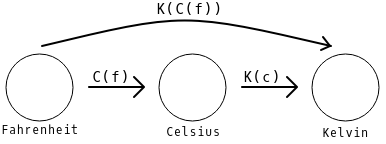
\includegraphics[width=0.6\textwidth]{./img/c5q5.png}
\end{figure}

Vamos explorar a fundo a ideia de funções compostas nas próximas questões.

\subsection*{Composição de funções}

Vamos voltar à notação tradicional de função.

\begin{shaded*}
A partir das funções $f(x)=2x+3$ e $g(x)=5^x$, podemos obter as seguintes composições:

$$ f \circ g = f(g(x)) = 2 \cdot 5^x + 3 $$
$$ g \circ f = g(f(x)) = 5^{2x+3}$$
\end{shaded*}

Para obter $f(g(x))$, que é o mesmo que $f \circ g$, devemos substituir a variável $x$ na função $f(x)$ pela função $g(x)$.

$$ f(x)=2x+3 \newline $$
$$ f(\mathbf{x})=2 \mathbf{x}+3  $$
$$ f(\mathbf{g})=2 \mathbf{g}+3  $$
$$ f(\mathbf{g(x)})=2 \mathbf{g(x)}+3  $$
$$ f(\mathbf{g(x)})=2 \cdot \mathbf{5^x}+3  $$
$$f(g(x))=2 \cdot 5^x+3  $$

Caso você não tenha entendido o que foi feito acima, sugerimos a leitura dos problemas 4, 5 e 6 a partir da página 350 do livro \sugestao{Matemática básica - volume 1}.

\begin{questao}
Responda aos itens abaixo considerando as duas funções usadas como exemplo logo acima.
\begin{enumerate}[a)]
\item Qual é o valor de $f(g(1))$?
\item Para qual valor de $x$ temos $f(g(x))=53$?
\item Qual é o valor de $g(f(1))$?
\item Para qual valor de $x$ temos $g(f(x))=5$?
\end{enumerate}
\end{questao}

É importante que esteja claro pra você que $f(g(x))$ e $g(f(x))$ são funções diferentes. Veja que os itens a e d acima resultaram em valores diferentes. Além disso, a expressão algébrica de $f(g(x))$ é diferente da de $g(f(x))$.

\subsection*{Descompondo funções}

Embora composição de funções seja fundamental para modelar fenômenos complexos, ao longo da disciplina de cálculo é bastante útil conseguir ``descompor'' uma função dada em duas funções mais simples.

Por exemplo, a função $f(x)=\sin(x^2-9)$ pode ser vista como uma composição das funções $g(x)=\sin(x)$ e $h(x)=x^2-9$. Nesse caso, $f(x)=g(h(x))$. Também poderíamos usar as funções $i(x)=\sin(x-9)$ e $j(x)=x^2$ e escrever corretamente que $f(x)=i(j(x))$. A escolha da primeira ou segunda composição depende dos seus objetivos. Em Cálculo, você usará essa estratégia para calcular a derivada de uma função, portanto, seu foco deve ser em quebrar a função em partes que você saiba derivar.

\begin{questao}
Escreva as funções abaixo como a composição de duas funções a sua escolha. Indique tanto as novas funções como a ordem em que foram compostas para obter a função dada.
\begin{enumerate}[a)]
\item $a(x)=3+\cos^2(x)$
\item $f(x)=\frac{1}{\sqrt{x-5}}$
\item $p(x)=3 \cdot 2^{x-1}$
\item $t(x)=(\sin(x)+1)(\sin(x)+2)$
\end{enumerate}
\end{questao}

\subsection*{Composição ou multiplicação}

Como dito anteriormente, o objetivo de descompor uma função dada nas disciplinas de cálculo é viabilizar o cálculo de derivadas (pela regra da cadeia) ou integrais. Porém, em alguns casos quebrar uma função dada como um produto de duas funções mais simples pode ser mais útil (graças à regra do produto).

Considere, por exemplo, a função $f(x)=(3x+1).\sin(x)$. Se tentarmos reescrevê-la como uma composição de duas funções, poderíamos usar $g(x)=3x+1$, mas a outra função precisaria ser $h(x)=x.\sin(\frac{x-1}{3})$ para que ao calcularmos $h(g(x))$ o argumento de $\sin$ fosse igual a $x$. Nesse caso, a decomposição da função não simplificou muito a função dada. Entretanto, poderíamos ver $f(x)$ como sendo o produto de $g(x)=3x+1$ e $i(x)=\sin(x)$, essas sim são funções mais simples de derivar ou integrar.

\begin{questao}
Rescreva as funções abaixo como a composição ou a multiplicação de outras duas funções mais simples.
\begin{enumerate}[a)]
\item $f(x)=x^2 \cdot 3^x$
\item $g(x)=\frac{x+3}{x+4}$
\item $p(x)=\cos(x^2-1)$
\item $m(x)=\frac{2^x}{1+2^x}$
\item $t(x)=x^2\sin(x)$
\end{enumerate}
\end{questao}

\subsection*{Uma composição especial}

\begin{questao}
Considere as funções $m(x)=2x-6$ e $n(x)=\frac{x}{2}+3$
\begin{enumerate}[a)]
\item Obtenha a expressão algébrica de $m(n(x))$.
\item Obtenha a expressão algébrica de $n(m(x))$.
\end{enumerate}
\end{questao}

Nos itens acima você deve ter obtido que $m(n(x))=x$ e $n(m(x))=x$. Toda função da forma $f(x)=x$ é chamada de identidade pois $f(1)=1$, $f(2)=2$, $f(3)=3$, $f(-17)=-17$ , $f(1000)=1000$... Quando a composição de duas funções é igual à identidade, dizemos que uma delas é a \textbf{função inversa} da outra. No caso da questão acima, dizemos que $m(x)$ é a função inversa de $n(x)$ e vice-versa. No caso geral, a inversa de uma função $f(x)$ é representada por $f^{-1}(x)$.

\subsection*{Funções inversas}

\begin{questao}
Utilize a expressão $C=\frac{5(F-32)}{9}$, dada no começo deste capítulo para converter uma temperatura em celsius para fahrenheits, para responder as questões abaixo.
\begin{enumerate}[a)]
\item Rescreva a fórmula acima isolando $F$ ao invés de $C$.
\item Use a resposta do item anterior para obter o valor em fahrenheits para a temperatura de 35\degree Celsius.
\end{enumerate}
\end{questao}

Agora pense nas fórmulas acima, a dada no enunciado e a obtida no item b, como funções. Podemos escrevê-las como $C(f)=\frac{5(f-32)}{9}$ e $F(c)=\frac{9c+160}{5}$. A primeira delas retorna uma temperatura em celsius a partir de um valor dado em fahrenheits. A segunda retorna um valor em fahrenheits a partir de um valor dado em celsius. Ou seja, elas fazem trabalhos inversos!

\begin{figure}[h]
\centering
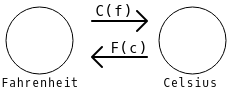
\includegraphics[width=0.5\textwidth]{./img/c5q9.png}
\end{figure}

Esse é justamente o significado de duas funções serem inversas. 

\begin{questao}
Verifique se a composição $C \circ F$ resulta na função identidade.
\end{questao}

\subsection*{Obtendo funções inversas} %%nao sei se mantenho essa

O exemplo acima nos oferece não apenas uma interpretação para funções compostas, mas também um método para obtê-las: se você quer obter a inversa de $f(x)$, isole a variável $x$ e obtenha uma expressão envolvendo $y$. Por exemplo, a inversa de $f(x)=2+\frac{1}{x}$ pode ser obtida da seguinte maneira:

\begin{align*}
 f(x) &=2+\frac{1}{x} && \text{por conveniência, vamos trocar } f(x) \text{ por } y \\
 y &= 2+\frac{1}{x} && \text{subtraindo 2 dos dois lados}\\ 
 y-2 &= \frac{1}{x}  && \text{invertendo os dois lados da igualdade}\\
 \frac{1}{y-2} &= x && \text{rescrevendo a igualdade}\\
 x &= \frac{1}{y-2}
\end{align*}

A expressão algébrica da função inversa foi obtida na última linha acima. Porém, escrevendo na forma convencional de funções, dizemos que a inversa de $f(x)$ é $f^{-1}(x)=\frac{1}{x-2}$. Usa-se $x$ como variável apenas por convenção, especialmente em casos em que as funções são dadas de forma não contextualizadas.

\begin{reflita}
Antes de resolver a questão abaixo, descreva com suas palavras como você deve proceder para resolvê-lo do início até a resposta final, dada no forma $f^{-1}$. 
\end{reflita}

\begin{questao}
Use a técnica discutida anteriormente para obter a função inversa das seguintes funções.
\begin{enumerate}[a)]
\item $f(x)=4x-8$.
\item $g(x)=\frac{3}{x-1}+2$.
\item $h(x)=3+log(2x)$.
\item $p(x)=\sin(3x-10)$.
\item $c(x)=2^{x+5}$.
\end{enumerate}
\end{questao}

\newpage

\section{Rumo ao livro-texto}

Nessa altura do curso de Cálculo, você já viu como derivar algumas funções, como as polinomiais e exponenciais.  Entretanto, uma função como $f(x)=2^{x^3+1}$, apesar de envolver uma exponencial e um polinômio, não se encaixa exatamente em nenhuma dessas categorias. Para esse tipo de situação, você estudará técnicas como a regra do produto, do quociente e da cadeia. A regra do produto (e do quociente) é útil para casos em que a função dada pode ser vista como um produto (ou quociente) de duas funções mais fáceis de derivar. A regra da cadeia permite calcular a derivada de uma função que possa ser decomposta em funções mais simples, lidando apenas com estas.

Não se preocupe em decorar a regra da cadeia ou entender os seus porquês neste momento, pois você terá aulas sobre ela em breve. Mas vejamos o que ela diz para resolver uma questão de um dos livros-texto.

\begin{shaded*}
Seja $f(x)$ uma função que pode ser decomposta em $g(h(x))$. Então, a sua derivada pode ser dada por:

$$f'(x) = h'(x) \cdot g'(h(x)) $$
\end{shaded*}

A questão abaixo foi retirada da seção 3.5 do livro \sugestao{Calculus}, de James Stewart.

\begin{resolvida}
Encontre a derivada de $y=10^{1-x^2}$.
\end{resolvida}

Note que a função dada não se enquadra em nenhum dos tipos de função básicos que você sabe como derivar. Porém, ela pode ser decomposta em uma exponencial simples ($f(x)=10^x$)e um polinômio ($g(x)=1-x^2$) e essas duas funções você já deve saber como derivar.

$$f'(x)=log(10) . 10^x $$
$$g'(x)=-2x $$

Agora, vamos checar a regra da cadeia tendo em mente que $y=f(g(x))$.

$$y' = g'(x) \cdot f'(g(x))$$

A primeira parte é simples, basta substituir $g'(x)=-2x$, resultando em $y' = -2x \cdot f'(g(x))$.

A segunda parte é a composição de $f'(x)$ com $g(x)$. Como $f'(x)=log(10) . 10^x$, temos que:

\begin{align*}
 f'(\mathbf{x}) &= log(10) . 10^\mathbf{x} \\
 f'(\mathbf{g(x)}) &= log(10) . 10^\mathbf{g(x)} \\
 f'(\mathbf{g(x)}) &= log(10) . 10^\mathbf{1-x^2} \\
\end{align*}

Portanto:

\begin{align*}
y' &= -2x \cdot log(10) . 10^\mathbf{1-x^2} && \text{rescrevendo o lado direito da igualdade} \\
y' &= -2log(10) \cdot x \cdot 10^\mathbf{1-x^2} \\
\end{align*}

Agora, tente aplicar a regra da cadeia para resolver a questão abaixo, também retirada do livro \sugestao{Calculus}, de James Stewart.

\begin{resolva}
Encontre a derivada de $y=e^{\sqrt{x}}$.
\end{resolva}

\newpage

\section{Gabarito}

Confira as respostas para as questões e \textbf{não se esqueça de registrar o seu progresso}.

\noindent\textbf{Questão 1:} a) $9$ e $4$, b) $\pm3$ e $\pm2$.

\noindent\textbf{Questão 2:} a) $0$, $2$ e $-2$, b) $14$ e $23$, c) $1$, d) $\pm2$, $\pm\sqrt{6}$.

\noindent\textbf{Questão 3:} a) $\frac{1}{t+2}$, b) $\frac{\sin(t)}{t}$, com $t=1/x$, c) $2t \cdot log(t)$, com $t=\sqrt{x}$.

\noindent\textbf{Questão 4:} a) $x=y-2$, b) $y^3-21y+20=0$.

\noindent\textbf{Questão 5:} a) $10\degree$ celsius, b) $283$ kelvin, c) $298$ kelvin, d) $K=\frac{5(F-32)}{9}+273$, e) $267$ kelvin.

\noindent\textbf{Questão 6:} a) $13$, b) $x=2$, c) $5^5$, d) $x=-1$.

\noindent\textbf{Questão 7:} a) $a(x)=b(c(x))$, $b(x)=3+x^2$ e $c(x)=cos(x)$, b) $f(x)=g(h(x))$, $g(x)=1/x$ e $h(x)=\sqrt{x-5}$, c) $p(x)=q(r(x))$, $q(x)=3.2^x$ e $r(x)=x-1$, d) $t(x)=u(v(x))$, $u(x)=x(x+1)$ e $v(x)=sen(x)+1$.

\noindent\textbf{Questão 8:} a) $f(x)=g(x).h(x)$, $g(x)=x^2$ e $h(x)=3^x$, b) $p(x)=q(r(x))$, $q(x)=\cos(x)$ e $r(x)=x^2-1$, c) $g(x)=h(x)/i(x)$, $h(x)=x+3$ e $i(x)=x+4$, d) $t(x)=u(x).v(x)$, $u(x)=x^2$ e $v(x)=sen(x)+1$, e) $m(x)=n(o(x))$, $n(x)=x/(1+x)$ e $o(x)=2^x$.

\noindent\textbf{Questão 9:} a) $m(n(x))=x$, b) $n(m(x))=x$.

\noindent\textbf{Questão 10:} a) $F=\frac{9C}{5}+32$, b) $95\degree$ fahrenheit.

\noindent\textbf{Questão 12:} a) $f^{-1}(x)=\frac{x+8}{4}$, b) $g^{-1}(x)=\frac{3}{x-2}+1$, c) $h^{-1}(x)=\frac{10^{x-3}}{2}$, d) $p^{-1}(x)=\frac{\arcsin(y)+10}{3}$, e) $c^{-1}(x)=log_2 (y)-5$.

\section{Registro de progresso}

Essa parte por enquanto fica com conteúdo vazio até que seja decidido como será feito o controle do progresso.

\newpage

\section{Auto-avaliação final}
Avalie o quanto você acha que sabe sobre os seguintes itens após ter resolvido as questões deste capítulo.

\begin{center}
 \begin{tabular}{|p{35mm}||p{15mm}|p{15mm}|p{15mm}|p{15mm}|} 
 \hline
   & Nada & Muito pouco & Noções gerais & Bastante\\
 \hline
 Usar troca de variáveis para resolver uma equação &  &  &  &  \\ 
 \hline
 Obter a composta de duas funções dadas &  &  &  &  \\
 \hline
 Obter a função inversa de uma função dada &  &  &  &  \\
 \hline
\end{tabular}
\end{center}

Cheque como foi o seu progresso comparando essas respostas com as que você deu antes de estudar este capítulo. Caso você não tenha atingido o nível ``Bastante''  em algum dos tópicos acima, liste abaixo qual ação concreta você fará nos próximos dias para atingi-lo:

\vspace{0.3cm}

\noindent\rule{\linewidth}{0.4pt}

\noindent\rule{\linewidth}{0.4pt}

\noindent\rule{\linewidth}{0.4pt}

\end{document}
